\documentclass[../part_1.tex]{subfiles}

\begin{document}
    \subsubsection{DINO}
    \par Задача \acrshort{mlm}, несмотря на свою эффективность в предобучении языковых моделей, не обеспечивает понимания текста в силу локального характера оптимизации, где модель предсказывает токены, не требуя анализа глобальных связей. Так же модель может правильно угадывать слово не понимая смысла текста.
    \par В последнее время большую популярность получил метод обучения \acrshort{dino}\cite{caron2021emergingpropertiesselfsupervisedvision, oquab2024dinov2learningrobustvisual, darcet2024visiontransformersneedregisters}, разработанный FacebookResearch. Это современный алгоритм самообучения, который позволяет эффективно извлекать универсальные признаки из изображений без использования размеченных данных. 
    \par Ключевая идея \acrshort{dino} -- принцип самодистеляции, где модель учится согласовывать представления одного изображения после различных аугментаций, формируя устойчивые и информативные представления. 
    \par Для обучения используется две модели -- учитель и ученик. Учитель генерирует эталонные представления изображения, тогда как ученик пытается предсказать выход учителя. Во время обучения изменяются исключительно параметры ученика, тогда как веса модели учителя вычисляются как экспоненциально взвешенное среднее весов ученика на каждой итерации, обеспечивая стабильное самообучение на неразмеченных данных.
    \begin{figure*}[h]
        \begin{subfigure}{0.33\textwidth}
            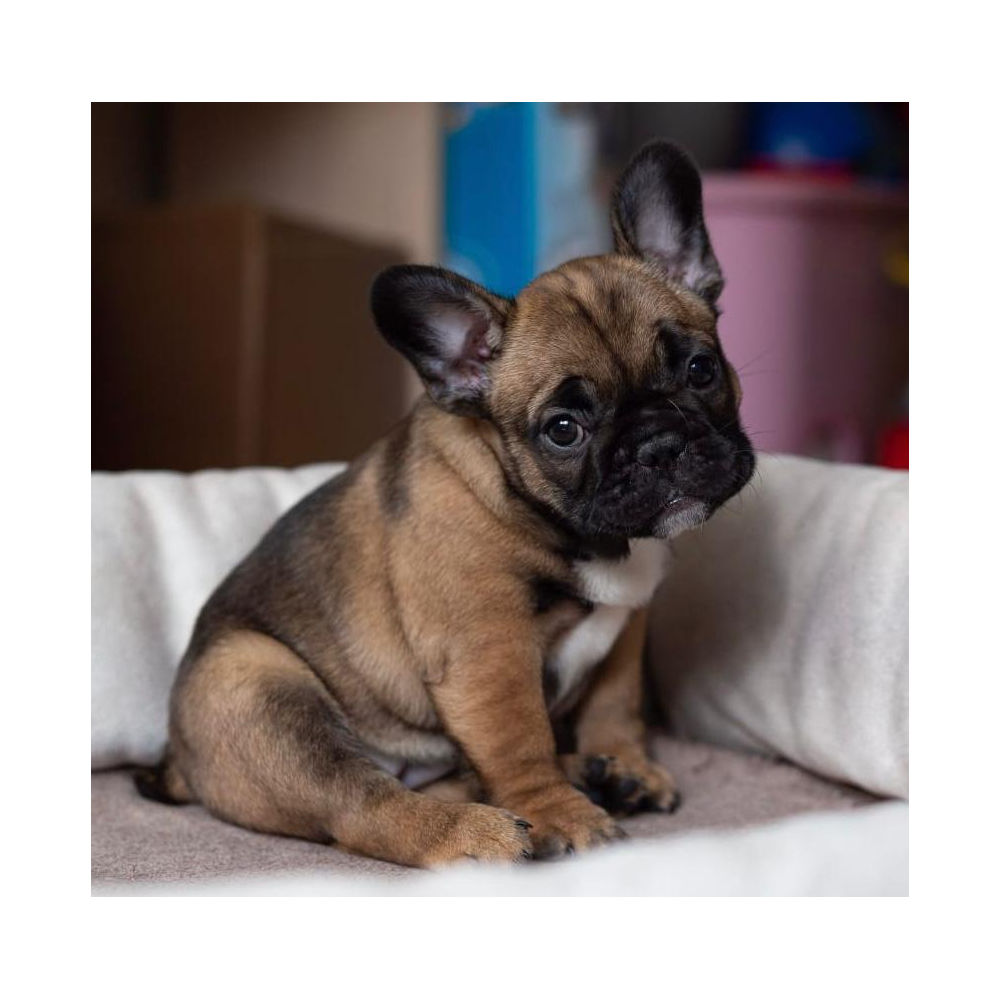
\includegraphics[width=\linewidth]{orig_image.png}
            \caption{Оригинальное изображение}
        \end{subfigure}%
        \hfill
        \begin{subfigure}{0.33\textwidth}
            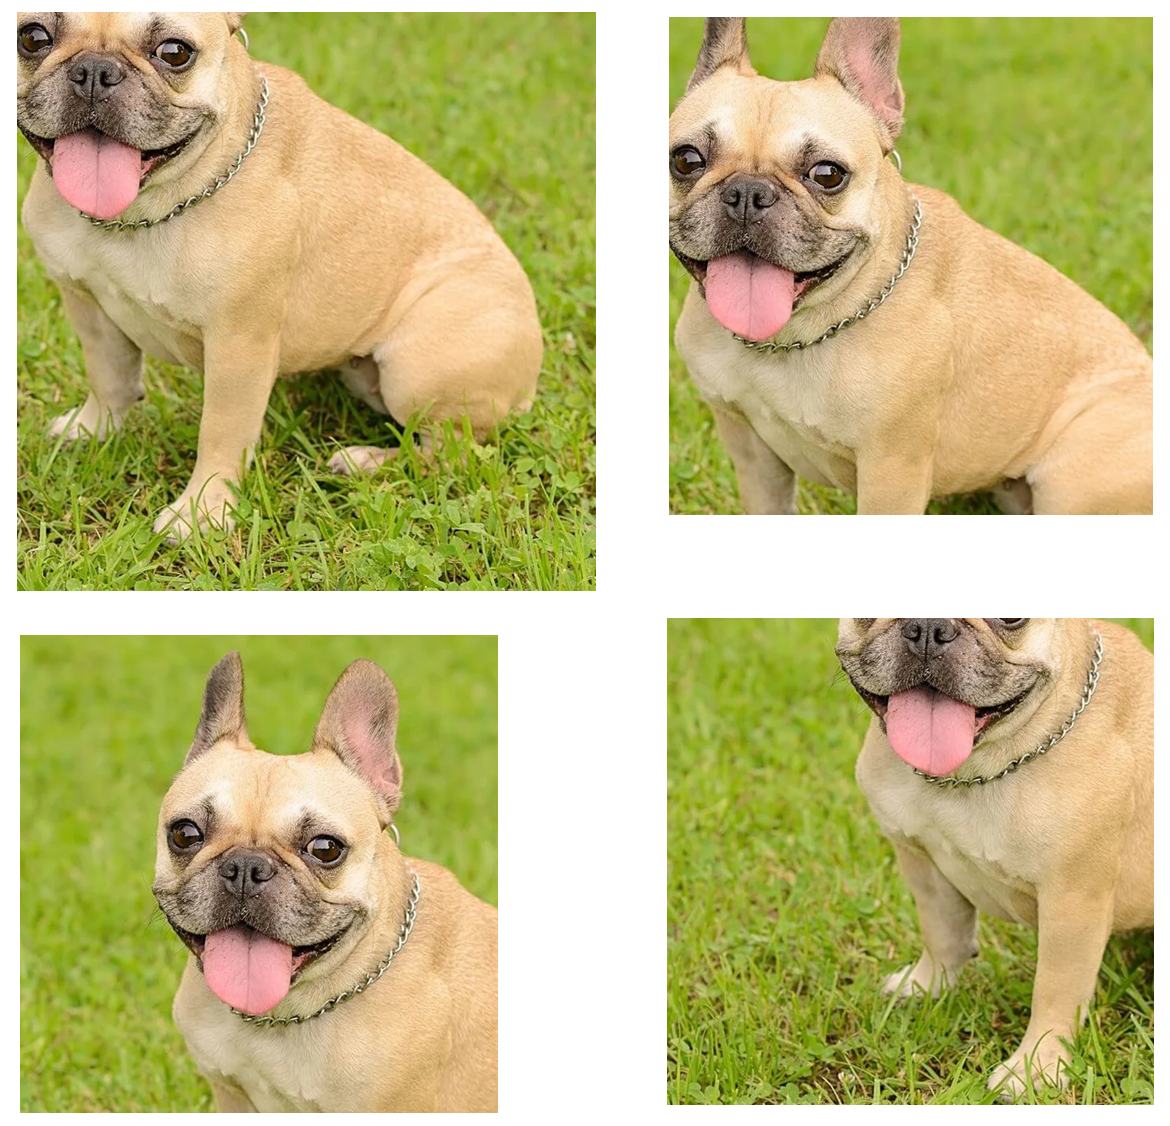
\includegraphics[width=\linewidth]{global_crops.png}
            \caption{Глобальные кропы}
        \end{subfigure}%
        \hfill
        \begin{subfigure}{0.33\textwidth}
            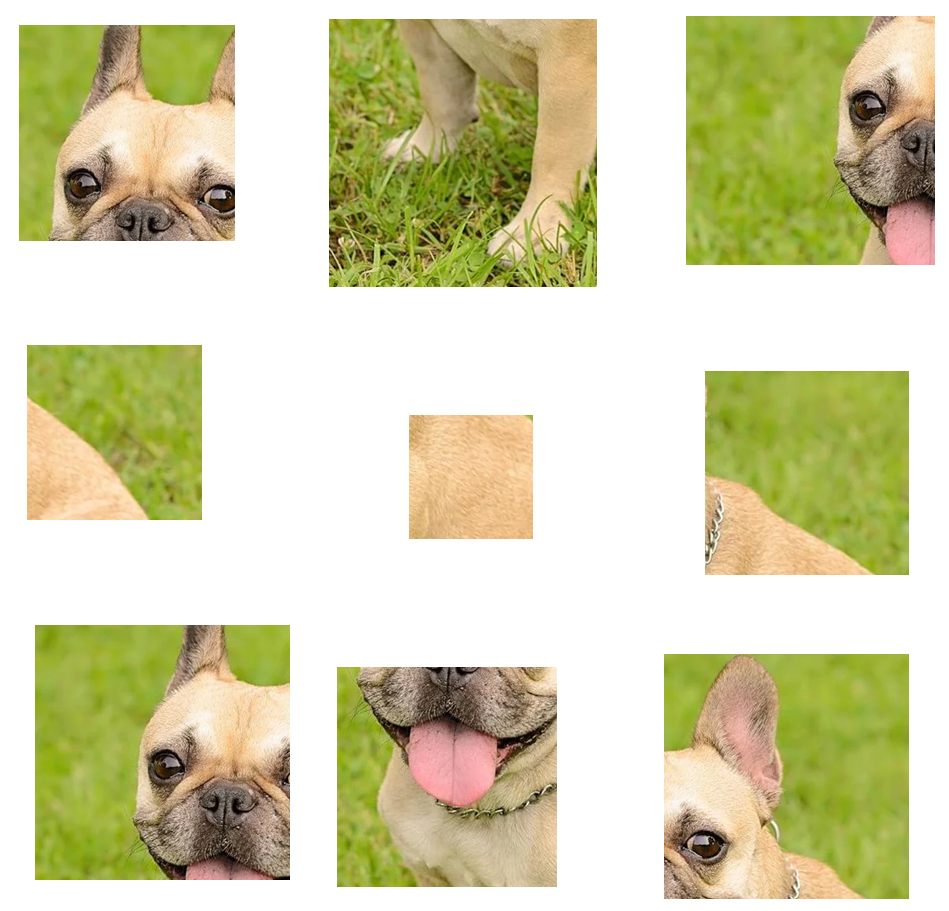
\includegraphics[width=\linewidth]{local_crops.png}
            \caption{Локальные кропы}
        \end{subfigure}%
        \label{fig:multicrop_augment}
    \end{figure*}
    \par Для того, чтобы избежать предсказания константы в \acrshort{dino} применяют центрирование. Из предсказания модели учителя вычитается скользящее среднее предыудщих предсказаний модели учителя. Центрирование смещает выход учителя так, чтобы среднее значение элементов вектора было близко к нулю, это раздвигает кластеры в пространстве признаков.
    \par Также в loss функции используется техника заострения(Sharpening), которая делает выходное вероятностное распределение более пиковым, уменьшая энтропию и подчеркивая наиболее вероятные классы
    \begin{equation}
        \label{sharpening}
        P(x)^{(i)} = \frac{\displaystyle exp\Bigg(\frac{g_\theta(x)^{(i)}}{\tau}\Bigg)}{\displaystyle \sum^K_{k=1}exp\Bigg(\frac{g_\theta(x)^{(k)}}{\tau}\Bigg)}\,.
    \end{equation}

    \begin{figure}[htbp]
        \centering
        \begin{subfigure}{.49\textwidth}
            \centering
            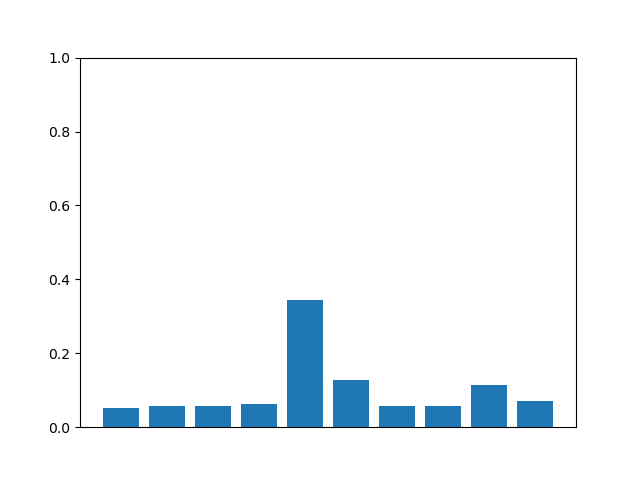
\includegraphics[width=.95\linewidth]{data.png}  
            \caption{Оригинальные данные}
        \end{subfigure}
        \hfill
        \begin{subfigure}{.49\textwidth}
            \centering
            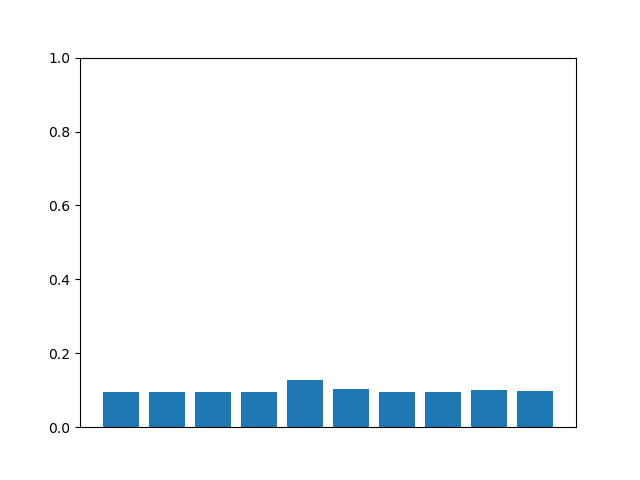
\includegraphics[width=.95\linewidth]{sharpend_1.png}  
            \caption{Данные после sharpening, $\tau = 1$}
        \end{subfigure}
        \vspace{1cm}
        \begin{subfigure}{.49\textwidth}
            \centering
            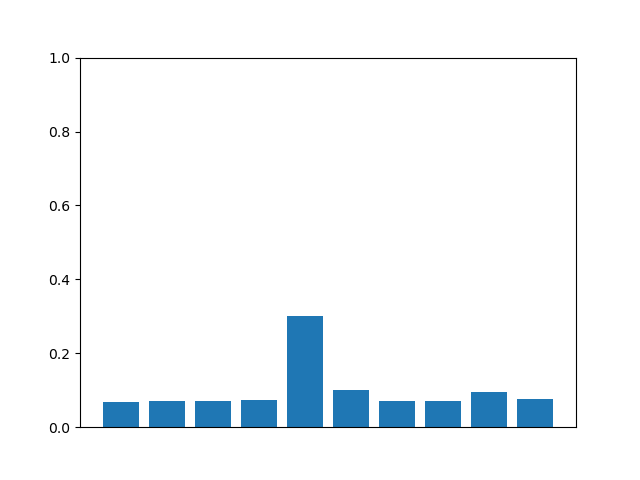
\includegraphics[width=.95\linewidth]{sharpend_0_2.png}  
            \caption{Данные после sharpening, $\tau = 0.2$}
        \end{subfigure}
        \hfill
        \begin{subfigure}{.49\textwidth}
            \centering
            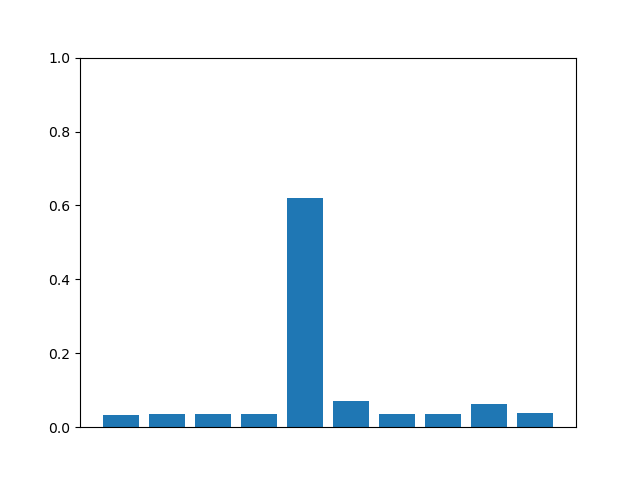
\includegraphics[width=.95\linewidth]{sharpend_0_1.png}  
            \caption{Данные после sharpening, $\tau = 0.1$}
        \end{subfigure}
        \caption{Распределение данных}
    \end{figure}

    \par Это помогает избежать тривиальных решений, когда модель вырождается  и предсказывает равномерное распределение для всех входов.
    \par В алгоритме \acrshort{dino} функцией потерь является кросс энтропия -- функция потерь, измеряющая расстояние между двумя распределениями вероятностей.
    \begin{equation}
        \label{cross_entropy}
        Loss = -P_t(x) \log P_s(x)\,.
    \end{equation}
\end{document}